\documentclass[a4paper]{article}

\usepackage[francais]{babel}
\usepackage[utf8]{inputenc}
\usepackage[OT1]{fontenc}
\usepackage{amsmath}
\usepackage{amssymb}
\usepackage{graphicx}
\usepackage{url}
\usepackage{subfigure}

\graphicspath{ {./imgs/} }

% shorten margin
\usepackage[]{fullpage}

\title{Configuration et sécurisation de services réseaux}
\author{Sophie VALENTIN, Mathieu BIVERT}

\makeatletter
\def\thickhrulefill{\leavevmode \leaders \hrule height 1pt\hfill \kern \z@}
\def\maketitle{
	\null
	\thispagestyle{empty}
	\vskip 1cm
	\begin{center}
		\normalfont\large\huge\@author
	\end{center}
	\vfil
	\vfil
	\vfil
	\vfil
	\vfil
	\vfil
	\vfil
	\vfil
	\vfil
	\vfil
	\vfil
	\hrule height 2pt
	\par
	\begin{center}
				\huge \strut \@title \par
				\@date
	\end{center}
	\hrule height 2pt
	\par
	\vfil
	\vfil
	\vfil
	\vfil
	\vfil
	\vfil
	\vfil
	\vfil
	\vfil
	\vfil
	\vfil
	\vfil
	\vfil
	\vfil
	\vfil
	\vfil
	\vfil
	\vfil
	\vfil
	\vfil
	\vfil
	\vfil
	\vfil
	\vfil
	\vfil
	\begin{center}
  			\huge Professeur : Bruno MARTIN
    \end{center}
	\null
	\begin{figure}[!ht]
		\centering
		
\includegraphics[scale=.5]{polytech.png}
	\end{figure}
	\vfil
	\cleardoublepage
}
\makeatother

\begin{document}
\maketitle

\newpage
\tableofcontents

\newpage

\section{Scénario}
Serveur « public » fournissant accès distant (VPN), compte email
(postfix, dovecot, client email), espace web (apache).

Encryption autant que faire ce peut.

Logs.

Outils d'audit.

\section{Topologie}
\section{Mise en place d'une passerelle et accès à Internet}
Une passerelle (gateway) est un homme du milieu reliant
deux réseaux distincts. Dans le cas présent, la machine \textit{passerelle}
doit faire communiquer les deux réseaux SLAN (192.168.1.0/24) et LAN Travaux 
Pratiques (192.168.2.0/24).

La passerelle doit être capable de transmettre des paquets IP :
\begin{verbatim}
  (passerelle)# echo 1 > /proc/sys/net/ipv4/ip_forward
\end{verbatim}

Afin de maintenir l'\textit{IP forwarding} après un reboot de la machine
\textit{passerelle}, on décommente dans le fichier \textit{/etc/sysctl.conf}
la ligne suivante :
\begin{verbatim}
  #net.ipv4.ip_forward=1
\end{verbatim}

\vspace{1\baselineskip}
L'IP Masquerade (Network Address Translation) doit être
activée. Cette fonctionnalité modifie les entêtes IPs du trafic
passant par \textit{passerelle} afin de rendre invisibles, au niveau IP,
les machines de LAN Travaux Pratiques depuis l'extérieur.
Ici on utilise du NAT dit de source utilisant la chaîne 
\textit{POSTROUTING} puisqu'on modifie les adresses sources du paquet.
\begin{verbatim}
  (passerelle)# iptables -t nat -A POSTROUTING -o eth0 -s 192.168.2.0/24 -j MASQUERADE
\end{verbatim}

Note : L'interface \textit{eth0} est connectée au réseau SLAN.

\vspace{1\baselineskip}
Enfin, syslogd doit être activé afin de logger les activités d'iptables

\begin{verbatim}
  (passerelle)# apt-get install inetutils-syslogd
  (passerelle)# edit /etc/syslog.conf # logs dans /var/log/kernel.log
  (passerelle)# services syslog
\end{verbatim}

\subsection{Tests}
On choisit un client, par exemple \textit{client-bsd}. On lui
retire l'interface réseau connectée à SLAN \textit{em0}, et on s'assure que
la machine est bien connectée sur LAN Travaux Pratiques via \textit{em1}, et
qu'elle peut communiquer avec la passerelle. 
\begin{verbatim}
  (client-bsd)# ifconfig em0 down
  (client-bsd)# ifconfig em1
  (client-bsd)# ping passerelle.cs.sr
\end{verbatim}

\vspace{1\baselineskip}
Puis, on configure la table de routage du client afin
que la route par défaut passe par \textit{passerelle} et on vérifie :
\begin{verbatim}
  (client-bsd)# netstat -r
\end{verbatim}
\begin{figure}[!ht]
	\centering
	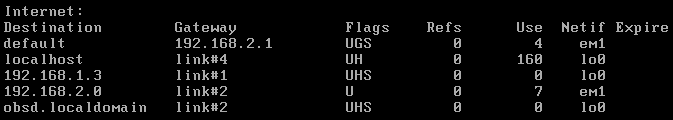
\includegraphics[scale=.5]{Internet.png}
	\caption{\label{routes} Table de routage de \textit{client-bsd}}
\end{figure}

\vspace{1\baselineskip}
Enfin, on s'assure qu'il est possible de contacter le serveur
 et d'atteindre Internet.
\begin{verbatim}
  (client-bsd)# ping -c3 google.fr
\end{verbatim}

\vspace{1\baselineskip}
On vérifie les logs sur la passerelle:
\begin{verbatim}
  (passerelle)# tail -f /var/log/kernel.log
\end{verbatim}

nmap ? Faire peut-être une partie "outils d'attaque et... d'audit"
où on explique l'utilisation de nmap, metasploit, vas (TP de demain)
et en quoi ils nous aident à sécu notre propre réseau.

\section{Mise à disposition d'un accès distant sur la machine et sécurisation}
Telnet, SSH, VPN
Expliquer comment mettre en place TCP Wrapper avec Telnet mais pas sécurisé.
essai ssh avec mitm? (normalement il affiche un message du genre
"SOMEONE MAY BE ON THE CABLE!")

\subsection{Serveur Telnet et attaques de \textit{sniffing}}

On commence par installer un serveur \textit{telnet} afin d'offrir
un premier accès distant à la machine \textit{passerelle}.

On n'utilisera pas ici le démon classique de telnet mais un démon
générique nommé \textit{inetd} permettant de minimiser le nombre
de processus lancés. Quand \textit{inetd} reçoit une demande 
de connexion, il lance le processus serveur adéquat. 

Pour ce faire, on installe le serveur telnet.
\begin{verbatim}
  (passerelle)# apt-get install telnetd
\end{verbatim}

Puis, on modifie le fichier \textit{/etc/inetd.conf} pour y
ajouter le service \textit{telnet} dans la section des services
standard, de façon à ce qu'il soit démarré automatiquement
en tant qu'utilisateur telnetd:
\begin{verbatim}
  (passerelle)# grep '^telnet' /etc/inetd.conf
  telnet        stream    tcp nowait telnetd /usr/sbin/tcpd /usr/sbin/in.telnetd
\end{verbatim}

\vspace{1\baselineskip}
On va maintenant tenter d'intercepter le couple \textit{login/passwd}
lors d'une connexion \textit{telnet} entre \textit{client-bsd}
et \textit{passerelle}.

Pour opérer, on utilise l'outil \textit{ettercap} depuis la machine BackTrack. 
Il faut le lancer ainsi :
\begin{verbatim}
  (backtrack)# ettercap -G
\end{verbatim}

\begin{enumerate}

\item Dans le menu, on clique tout d'abord sur \textit{Sniff} et on sélectionne 
\textit{Unified sniffing} avant de choisir l'interface \textit{eth1}
qui est sur LAN Travaux Pratiques.

\item Dans le menu \textit{Hosts}, on lance un scan du réseau local puis
depuis le même menu, on affiche la liste des hôtes.

\begin{figure}[!ht]
	\centering
	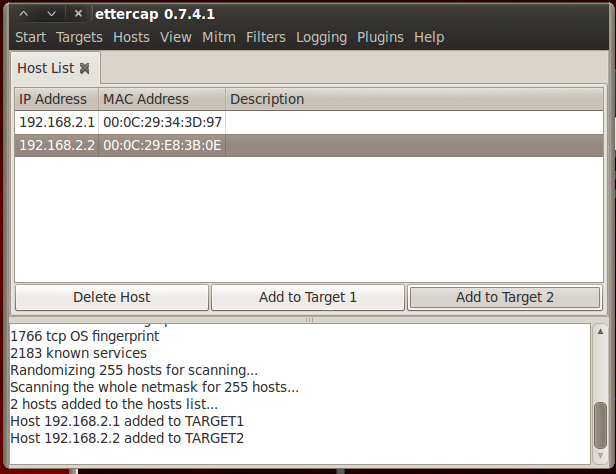
\includegraphics[scale=.4]{Hosts.PNG}
	\caption{\label{hosts} Hôtes détectés par le scan}
\end{figure}

On reconnaît les adresses IP de \textit{passerelle} et 
\textit{client-bsd}. Il suffit donc de spécifier que ce sont
nos deux cibles avec les boutons \textit{TARGET 1} et \textit{TARGET 2}.

\item Comme il s'agit d'un réseau commuté, on doit empoisonner les tables
ARP (\textit{ARP poisoning}) avant de lancer le \textit{sniffing} pour
récupérer le trafic entre les deux cibles.

Dans le menu \textit{Mitm}, on sélectionne donc \textit{ARP Poisoning}.

\item Enfin, on sélectionne dans le menu \textit{Start} le choix \textit{Start Sniffing}.

\end{enumerate}

La machine \textit{client-bsd} se connecte avec \textit{telnet}.

\begin{figure}[!ht]
	\centering
	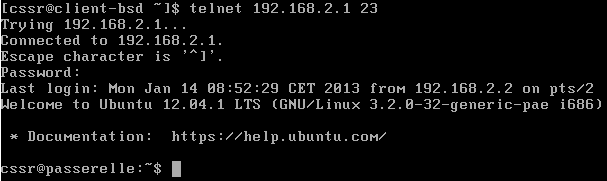
\includegraphics[scale=.5]{Telnet.PNG}
	\caption{\label{hosts} Connexion à \textit{passerelle}}
\end{figure}

Et on constate qu'il est extrêmement facile d'obtenir le couple \textit{login/password} en clair:

\begin{figure}[!ht]
	\centering
	
\includegraphics[scale=.5]{Telnet_passwd.png}
	\caption{\label{hosts} Couple en clair}
\end{figure}

On ne veut donc pas proposer un service d'accès à distance non sécurisé, c'est-à-dire
basé sur des communications transmises en clair sur le réseau. 

 
\subsection{Serveur SSH  et optimisations}
SSH (Secure SHell) joue un rôle similaire à telnet, mais contrairement à ce
dernier, il intègre des mécanismes de sécurité, comme l'encryption des
communications.

On installe puis démarre un serveur ssh sur la plateforme:
\begin{verbatim}
  (passerelle)# apt-get install openssh-server
  (passerelle)# service ssh start
\end{verbatim}

On teste une connexion avec mot de passe (l'option \textit{-v} est
utilisé pour montrer la différence avec une connexion à base de
clefs, voir plus bas)
\begin{verbatim}
  (client-bsd)$ ssh -v cssr@passerelle.cs.sr
  <METTRE L'OUTPUT ICI>
\end{verbatim}

Afin d'éviter d'avoir à entrer le mot de passe à chaque connexion, on peut
utiliser un système à base de clefs. On génère un couple clef privée/publique
de type RSA sur le client:
\begin{verbatim}
(client-bsd)$ ssh-keygen -t rsa
Generating public/private rsa key pair.
Enter file in which to save the key (/home/cssr/.ssh/id_rsa): 
Enter passphrase (empty for no passphrase): 
Enter same passphrase again: 
Your identification has been saved in /home/cssr/.ssh/id_rsa
Your public key has been saved in /home/cssr/.ssh/id_rsa
The key fingerprint is:
f4:3e:54:9f:df:eb:72:cc:7a:da:29:a5:79:58:0c:44 cssr@client-bsd
The key's randomart image is:
+--[ RSA 2048]----+
|            .E   |
|             .   |
|        .   o    |
|       . . . o . |
|        S o   =  |
|         o     =.|
|          o   O o|
|           . *.*o|
|             oX= |
+-----------------+
\end{verbatim}

Deux fichiers sont alors générés :
\begin{description}
	\item[id\_rsa.pub]	Clé publique devant être connue du serveur;
	\item[id\_rsa] 		Clé privée ne devant pas être dévoilée.
\end{description}

Côté serveur, on doit maintenant ajouter la clef publique sur le
serveur. SSH cherche dans le répertoire \textit{\$HOME/.ssh/} les
fichiers dont le nom commence par \textit{authorized\_keys}. Ceux-ci
doivent contenir une clef par ligne.

On transmet ainsi la clé publique sur le serveur, par exemple avec
\textit{scp}:
\begin{verbatim}
  (client-bsd)$ scp .ssh/id_rsa.pub cssr@passerelle.cs.sr:~/.ssh/authorized_keys2
\end{verbatim}

On prend soin d'ajuster les permissions du fichier :
\begin{verbatim}
  (passerelle)# chmod 700 authorized_keys2
\end{verbatim}
 
Enfin, on s'assure que l'authentification par clefs marche bien, et
qu'il est difficile de récupérer les informations sur la connexion
avec une attaque MITM.

La configuration du serveur SSH se fait dans le fichier \textit{/etc/ssh/sshd\_config}.
Il peut-être intéressant d'y faire les réglages suivants:
\begin{description}
	\item[X11Forwarding no] pour réduire le traffic X$11$, et donc réduire les
	risques de sécurité;
	\item[PermitRootLogin no] pour désactiver un accès distant direct au compte
	root;
	\item[Port 42], où tout autre port différent du port $22$ pour éviter les
	tentatives de connexions lancées par des bots.
\end{description}

\section{Configuration d'un serveur web et d'OpenSSL}
\subsection{Installation d'OpenSSL}
\begin{verbatim}
  (passerelle)# ./configure --prefix=/usr/local && make && make install
  (passerelle)# cat >> /etc/ld.so.conf
  /usr/local/openssl/lib
  ^D
  (passerelle)# ldconfig
\end{verbatim}

\subsection{Installation d'Apache2}
Après avoir récupéré les sources sur le site (et vérifié le hash du fichier), on configure
Apache avec le support d'OpenSSL
\begin{verbatim}
  (passerelle)# ./configure --option-du-chemin-ssl=/usr/local/openssl --prefix=/usr/local/apache2
  (passerelle)# /usr/local/bin/apache2/bin/apachectl start
  (passerelle)# wget http://localhost -O /dev/stdout && echo OK
\end{verbatim}

\subsection{Passage à https}

\subsection{Tests}

\section{Configuration serveur (smtp+imaps) et client (gpg) email}
\begin{figure}[!ht]
	\centering
	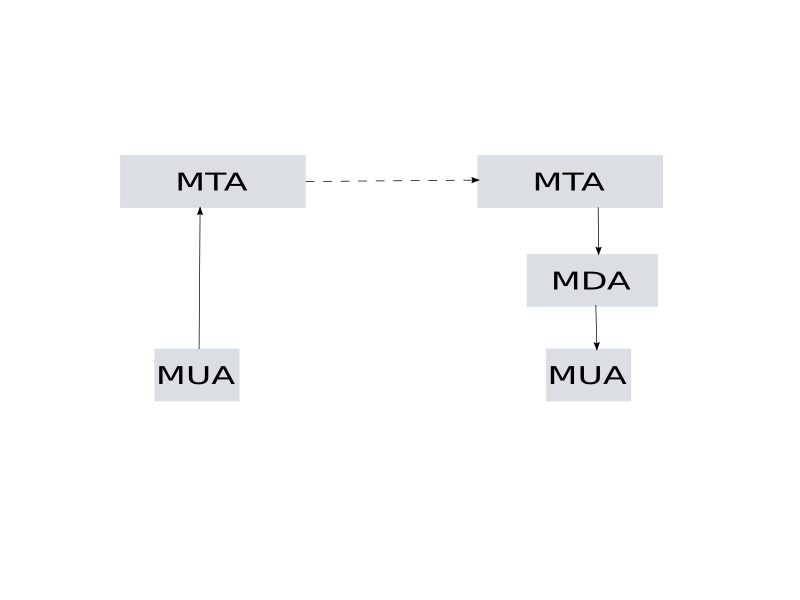
\includegraphics[scale=.5]{emailrouting.png}
	\caption{\label{emailrouting} Un MUA envoie un email à un MTA, qui
		le forward jusqu'à un MTA final, qui le transmet à un MDA.
		Enfin, le MUA du destinataire récupère l'email depuis ce MDA}
\end{figure}

La figure \ref{emailrouting} donne un exemple simple de routage d'email,
faisant intervenir $3$ pièces logicielles:
\begin{description}
	\item[MTA] Mail Transfer Agent (eg. serveur SMTP), qui route les
		emails de domaines en domaines jusqu'à arriver à bonne destination;
	\item[MDA] Mail Delivery Agent (eg. serveur IMAP(s)), qui délivre
		les emails aux MUAs qui lui demandent;
	\item[MUA] Mail User Agent c'est le client email, dont le rôle principal
		est de récupérer les emails depuis un MDA, et d'en envoyer à un MTA;
\end{description}
D'autres agents optionnels peuvent venir s'y greffer.

En pratique, on installe et configure postfix sur \textit{passerelle}.

\subsection{Tests}

\section{Configuration VPN}
\subsection{Tests}

\section{OpenVAS \& Metasploit}

\end{document}
